%!TEX root = ../../common/main.tex

\chapter{Conclusion and Outlook}
\label{ch:conclusion}

The \acl{SM} \dots

% SM, open questions, matter-antimatter asymmetry, LHCb built to test SM by precision measurements, CPV in BdToJpsiKS, golden channel, S and C, dataset, trigger, selection, tagging, acceptance, systematic effects, results:

The measurement of the \CP parameters \SJpsiKS and \CJpsiKS presented in this
thesis was realised on a dataset corresponding to an integrated luminosity of
$\SI{3.0}{\per\femto\barn}$ recorded by the \LHCb experiment in
\acl{protonproton} collisions at centre-of-mass energies of $\num{7}$ and
$\SI{8}{\TeV}$. The sample contains $\num{41500}$ reconstructed $\BdToJpsiKS$
candidates with a flavour tagging decision assigned by either the combination of
the \acl{OS} tagging algorithms or by the \acl{SSpi} tagging algorithm. Using an
\acl{uEML} fit the \CP parameters \SJpsiKS and \CJpsiKS are measured to be
%
\begin{equation*}
  \begin{split}
    \SJpsiKS &= \phantom{-}\num{0.731} \pm \num{0.035} \statp \pm \num{0.020} \systp \eqcm\eqand \\
    \CJpsiKS &=           \num{-0.038} \pm \num{0.032} \statp \pm \num{0.005} \systp \eqcm
  \end{split}
\end{equation*}
%
with a statistical correlation coefficient of $\rho(\SJpsiKS,\CJpsiKS) =
\num{0.483}$. With the parameter \CJpsiKS fixed to zero the measurement yields
$\SJpsiKS = \sintwobeta = \num{0.746 +- 0.030}\statp$.

The measurement improves the previous \LHCb result \cite{Aaij:1497268} by
including a larger dataset, additional trigger lines, an optimised candidate
selection and by incorporating the \SSpi tagger decisions. It is by now the most
precise measurement of \CP violation at a hadron collider and is in excellent
agreement with the current world average. \Cref{fig:conclusion:ckm_fitter_15}
shows the ${(\dquark,\bquark)}$ unitarity triangle in the
${(\ovE{\rho},\ovE{\eta})}$-plane from a global fit incorporating all measured
\CKM parameters \cite{Charles:2004jd} except from the one reported here that is
additionally shown to allow for a better comparison.
%
\begin{figure}[ht]
\centering
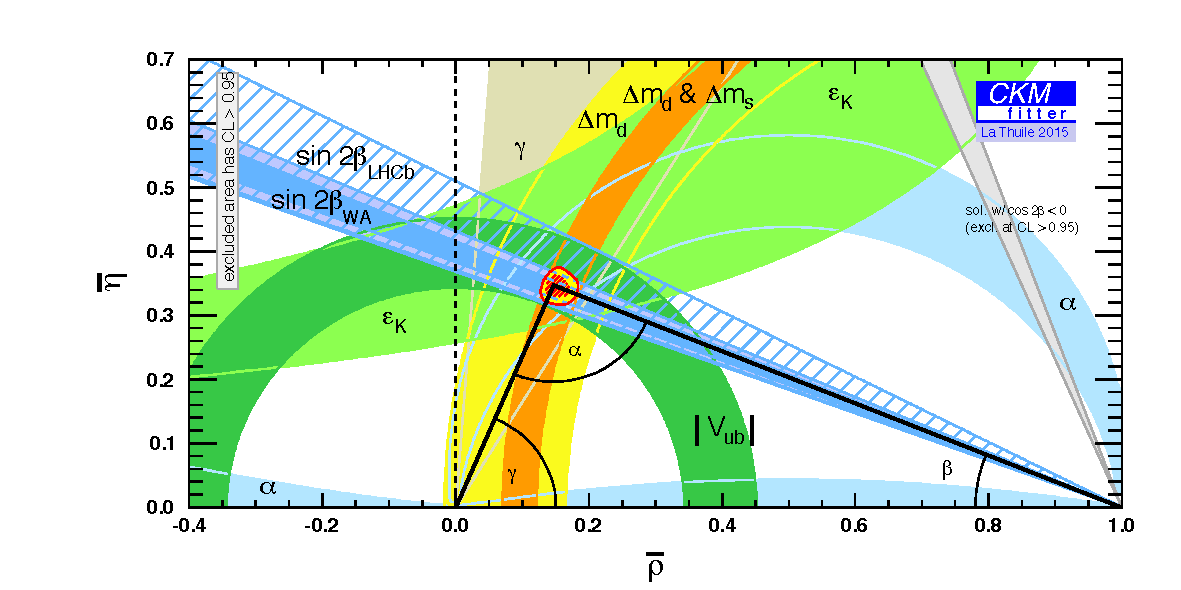
\includegraphics[width=1\textwidth]{private/content/conclusions/figs/ckmfitter_summer15.pdf}
\caption{Constraints on the ${(\dquark,\bquark)}$ unitarity triangle in the
${(\ovE{\rho},\ovE{\eta})}$-plane from a global fit incorporating all measured
\CKM parameters \cite{Charles:2004jd} except the results presented in this
thesis that is shown by itself as a comparison in light blue. Regions outside
the coloured areas have $1-p > \SI{95.45}{\percent}$. The red hashed region of
the global combination corresponds to $\SI{68}{\percent}$ \acp{CL}.}
\label{fig:conclusion:ckm_fitter_15}
\end{figure}


% global picture, UT fit tensions, Belle II prospects

% next steps: additional charmonium channels: Jpsi to e+e-, psi(2S)

% outlook to Run II and LHCb upgrade

\begin{figure}
  \centering
  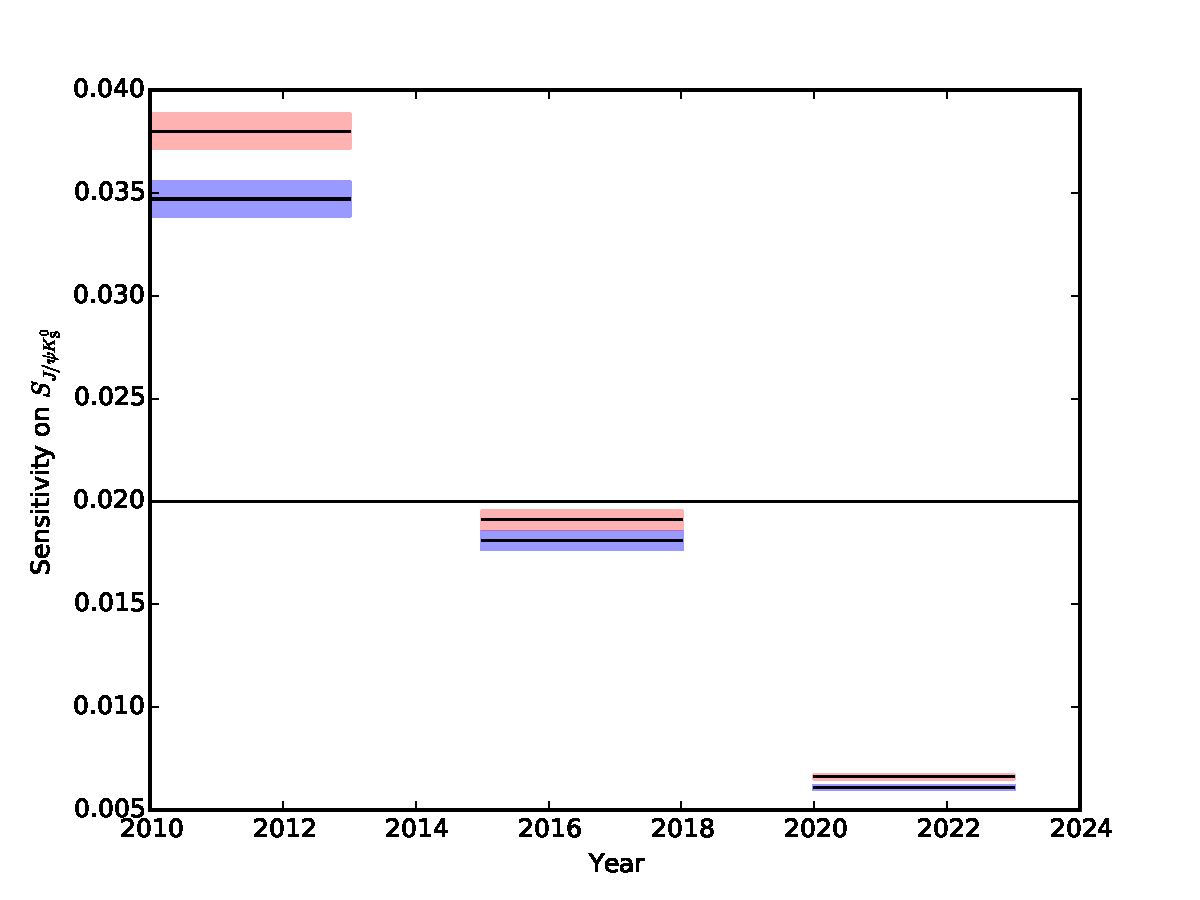
\includegraphics[width=1.00\textwidth]{private/content/conclusions/figs/comparison_of_significance.pdf}
  \caption{. \cite{Moedden:2015}}
  \label{fig:conclusion:upgrade:significance}
\end{figure}
